\documentclass{article}
\usepackage{import}
\import{../../template/}{article-template}
\graphicspath{{../../images/}}
\addbibresource{../../template/library.bib}

\usepackage{tikz}
\usepackage{showexpl}
\lstset{
    basicstyle=\ttfamily\small,
    explpreset={pos=b,rframe={},columns=flexible}
}

\title{LaTeX}
\author{PENG}
\date{\today}
\begin{document}
\maketitle
\tableofcontents
\section{Introduction}
\url{https://latex-project.org/}

\section{TikZ}
\subsection{Introduction}
\url{https://tikz.dev/}
\begin{definition}[TikZ]
    TikZ is a frontend of PGF.
\end{definition}

\subsection{Curved Path Construction}
\begin{definition}[control points]
    \verb|<ps> .. controls <pc1> and <pc2> .. <pe>|
\end{definition}

\begin{LTXexample}
    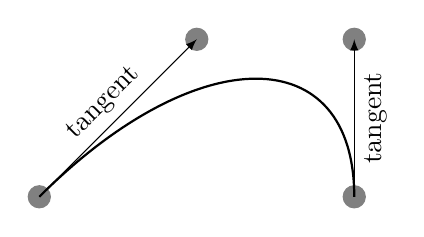
\begin{tikzpicture}[scale=2]
        \filldraw [gray]
        (0,0) circle (2pt)
        (1,1) circle (2pt)
        (2,1) circle (2pt)
        (2,0) circle (2pt);
        \draw [thick] (0,0) .. controls (1,1) and (2,1) .. (2,0);
        \draw [-latex] (0,0) -- node[sloped,above] {tangent} (1,1);
        \draw [-latex] (2,0) -- node[sloped,below] {tangent} (2,1);
    \end{tikzpicture}
\end{LTXexample}

\printbibliography
\end{document}